\chapter{Motivation and Approach}

\section{Adaptive sampling: Motivation}
Physical systems come in many forms and shapes and show an intrinsic hierarchical organization. Molecular dynamics (MD) simulations have become indispensable for gaining
insight into molecular systems at high spatial and temporal resolutions.
However, a fundamental limitation for MD with accurate all-atom force-fields remains
the computational demand for simulating processes with long timescales. In
particular, biologically relevant processes, such as protein folding and
conformational changes, typically require simulation time orders of magnitule longer than
milliseconds, while atomic-resolution MD trajectories can currently reach
timescales on the order of milliseconds on available computational resources. 

This thesis is about solving the challenge of accurately determining the conformational dynamics of high-dimensional stochastic systems. This method is especially useful in the context of molecular dynamics (MD) of proteins. Proteins and the obtaining of accurate stationary and kinetic behavior of protein is a crucial unsolved challenge that limits our understanding of the behavior of many systems. This includes the majority of biological processes. Such a broad challenge requires many hierarchical approaches. Adaptive sampling is one of these approaches, which build on to of hardware advances and software advances of the molecular dynamics engines.

\section{Outline}
 
 Overall this Dissertation resulted in several peer-reviewed publications \cite{Adstrategies2018, Extasy2016}, as well one publication under review \cite{Extasy2019}. The results obtained during my dissertation as well the results in the papers will be presented in the next chapters.
 
Chapter 2 will summarize some of the standard techniques, which will be used frequently throughout the thesis. While some of these approaches are commonly used in this field, there are also recently developed techniques which are less commonly used. The relevence of all these techniques for adaptive sampling will be highlighted. 

The theory of Adaptive sampling will be discussed in Chapter 3, as well the derivation of the first upper limit of the adaptive sampling speed up will be show. This novel result shows that adaptive sampling can be further improved. 
In the next chapter 4 the current strategies will be compared in statistically robust way and the effectivity of each strategy will be compared for different proteins and different goals.

Chapter 5will introduce the computational tools and software frame works necessary to successfully and efficiently execute adaptive sampling. Due to the many subtasks adaptive sampling consists off, these practical consideration have a direct impact on the viability of adaptive sampling for solving sampling problems.

This developed software framework will be used in Chapter 6 to show for different biomolecular systems the results and the accuracy which adaptive sampling can achieve. 

A final chapter will summarize the current achievements and discuss further open questions and possible directions.


\afterpage{\null\newpage}
\chapter{Background\label{sec:background}}

\section{Proteins and Molecular Dynamics (MD)}

The behavior of a protein or any biomolecule can be relatively accurately represented by Newton's classical equations of motion of all atoms. All 3N atom coordinates including the surrounding water solvent are represented by $\mathbf{x}_{t}$ positions and $\mathbf{v}_{t}$ velocities. The Newton's classical equations of motion are:

$$M\ddot{x_{t}}=-\nabla U(\mathbf{x}_{t})$$
The Hamiltionian $U()$ represents the all-atom force field guiding. The straightforward approach of numerically solving this equation leads to a molecular dynamics (MD) trajectory describing the motion of a protein. This Hamiltonian approximates the quantummechanics dynamics of the protein and is continously improved. Increased accuracy compared to the all-atom approach would require a quantummechanical approach, which reduces the reacheble timescales by several order of magnitude.  In this thesis the CHARMM22* force field \cite{Charmm22star} with modified TIP3P water was utilized.

\begin{figure}[H]
  \centering
  \begin{subfigure}[t]{0.45\textwidth}
    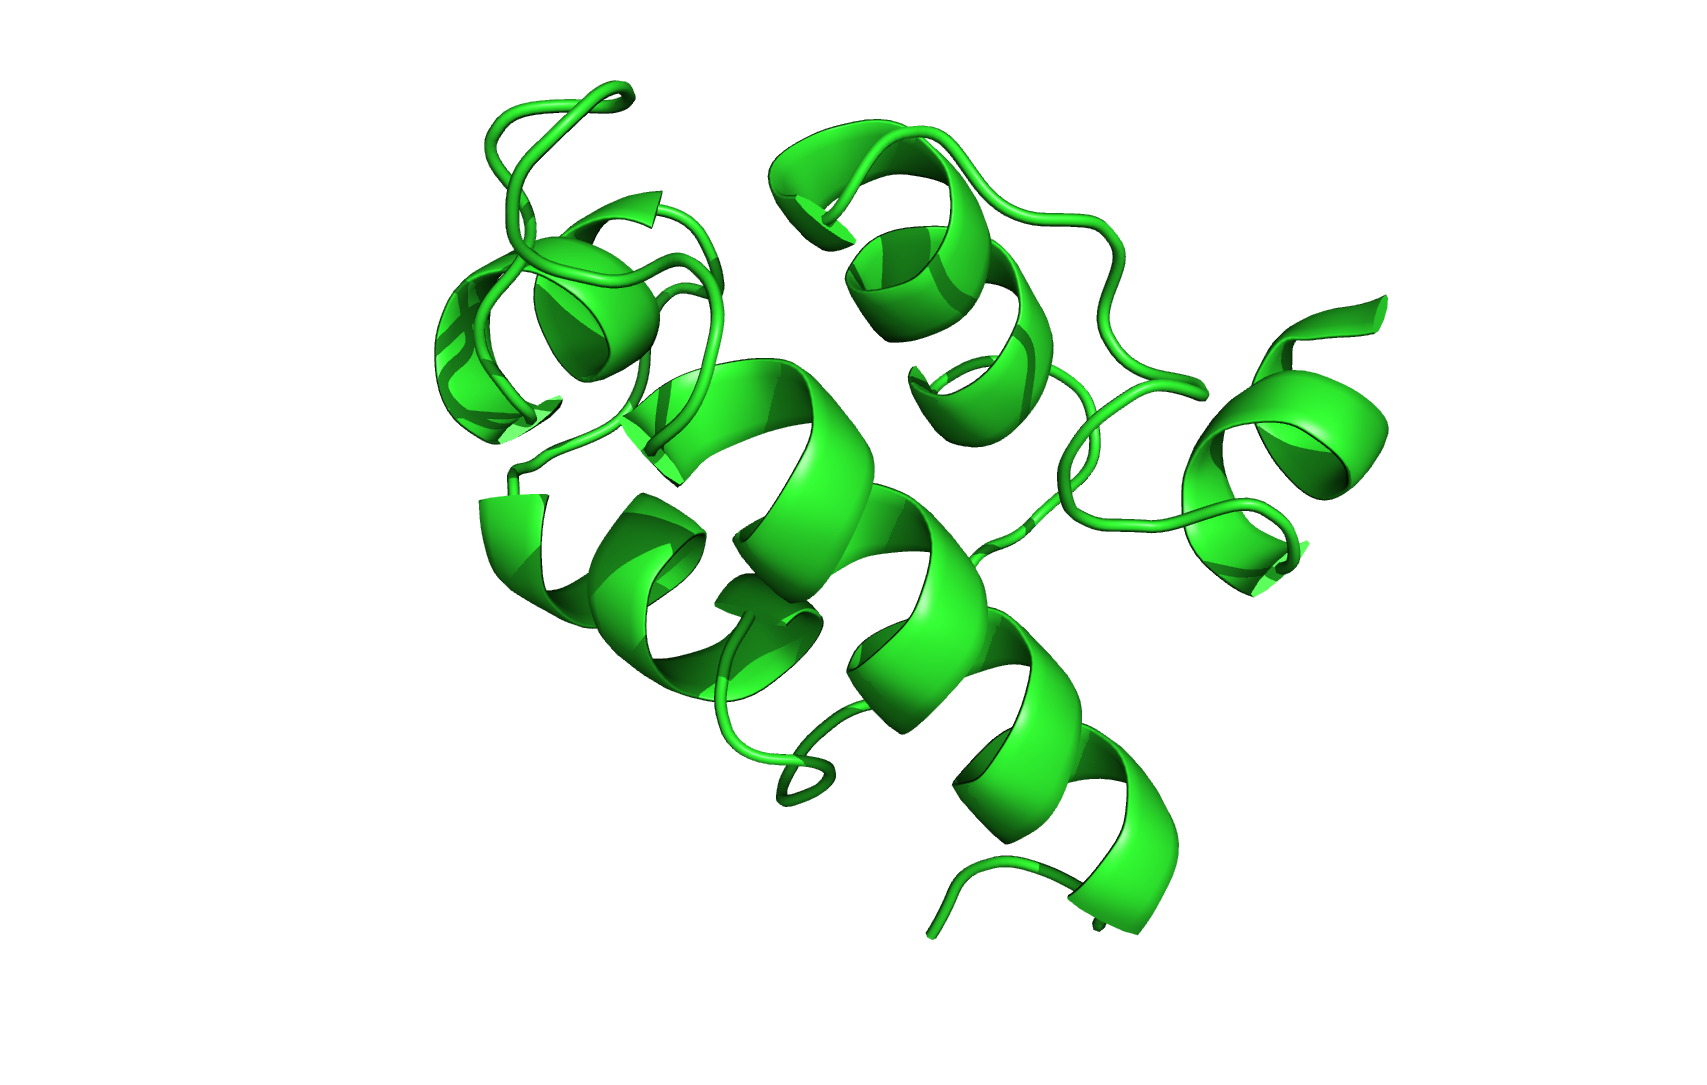
\includegraphics[width=0.9\textwidth]{figures3/lambda-repressor.png} 
  \end{subfigure}
  \begin{subfigure}[t]{0.45\textwidth}
    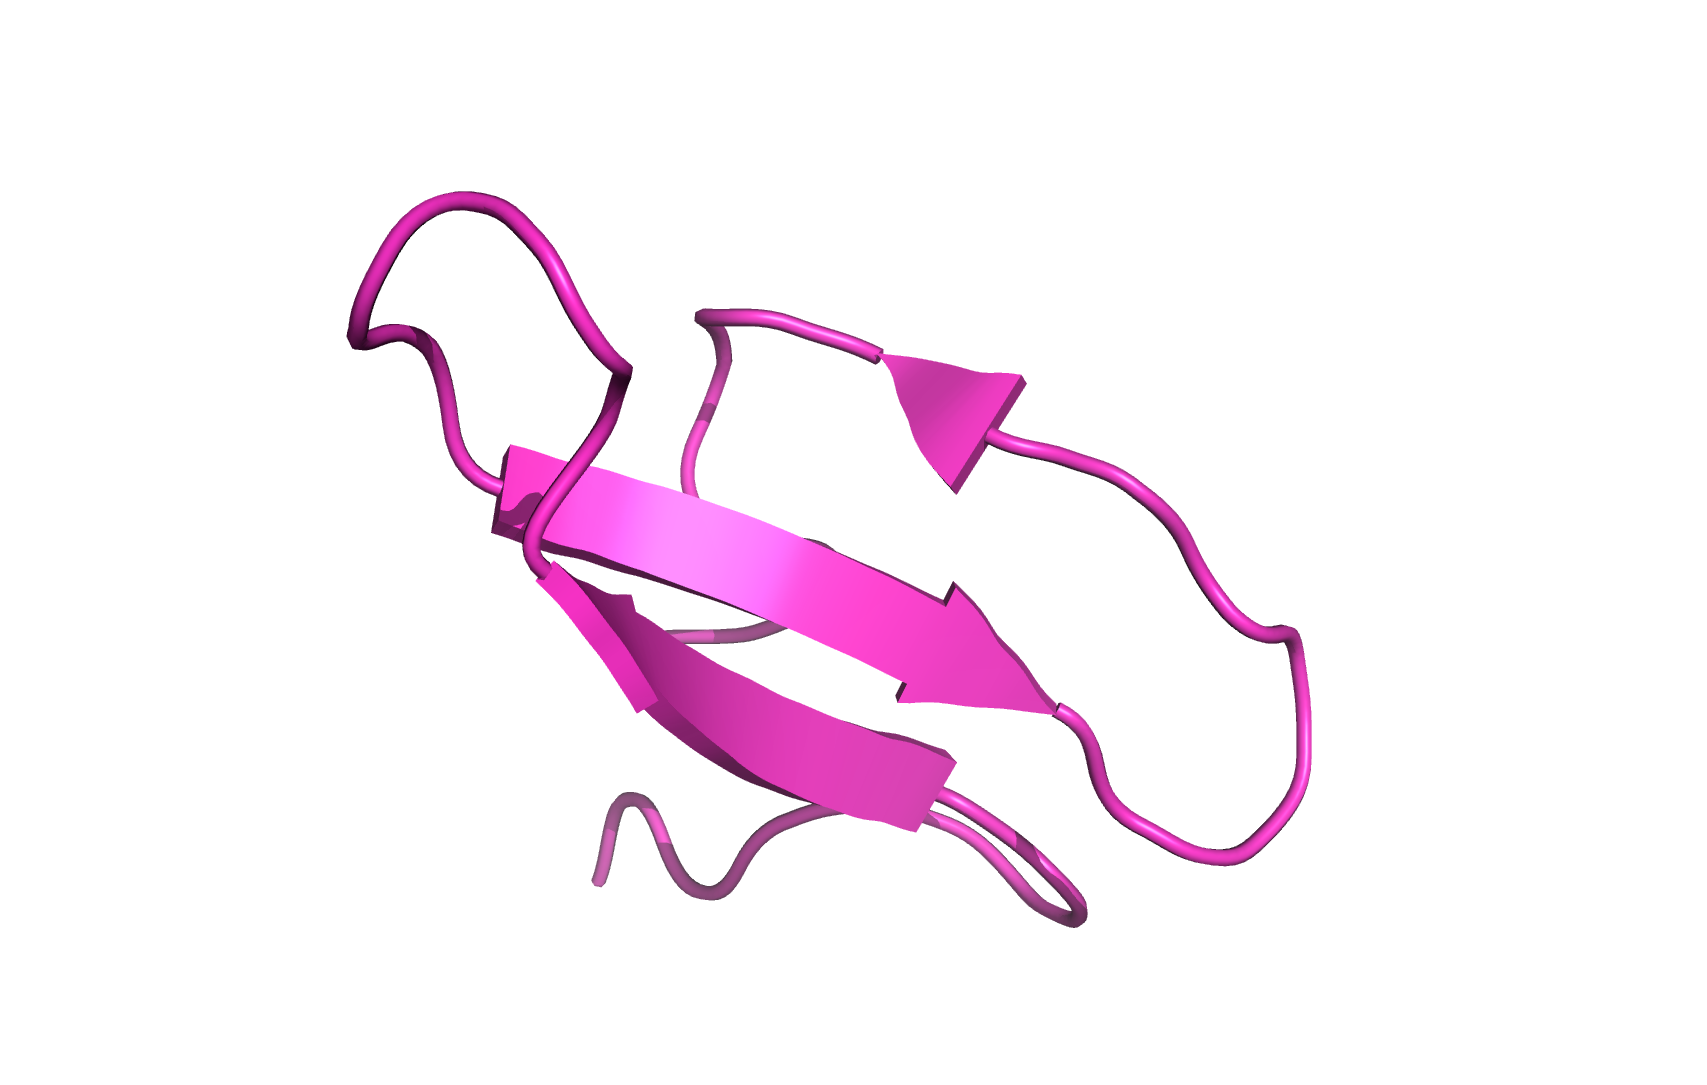
\includegraphics[width=0.9\textwidth]{figures3/ww-domain.png}  
  \end{subfigure}
  \caption{Structure of proteins $\lambda$-repressor and WW domain.}
  \label{fig:NN}
\end{figure}


The CHARMM force field has the following hamiltonian and consists of terms for molecular bonds stretching, angle bending, dihedral and improper dihedral energy terms, the Urey-Bradley component, van der Waals interactions (Lennard-Jones) and Coulomb interactions. 

$$U_{CHARMM}=U_{bonds}+U_{angle}+U_{dihedral}+U_{improper}+U_{UB}+U_{LJ}+U_{elec}$$

\begin{equation}
\begin{aligned}
U(r_{i})={} &\sum_{bonds}K_{b}(b-b_{0})^{2}+\sum_{angles}K_{\theta}(\theta-\theta_{0})^{2}+\sum_{torsions}K_{\phi}\left(1+cos(n\phi-\delta)\right)\\
&+\sum_{impropers}k_{\omega}\left(\omega-\omega_{0}\right)^{2}+\sum_{Urey-Bradley}k_{u}\left(u-u_{0}\right)^{2}\\
&+\sum_{nonbonded}\epsilon\left[\left(\frac{R_{min,ij}}{r_{ij}}\right)^{12}-\left(\frac{R_{min,ij}}{r_{ij}}\right)^{6}\right]+\sum_{electric}\frac{q_{i}q_{j}}{\epsilon r_{ij}}
\end{aligned}
\end{equation}

Here the parameters are: $k_b$ is the bond force constant, $b-b_0$ is the atom distance from equilibrium, $k_\theta$ is the angle force constant, $\theta-\theta_0$ is the angle from equilibrium between 3 bonded atoms, $k_\phi$ is the dihedral force constant, $n$ is the multiplicity of the dihedral function, $\phi$ is the dihedral angle, $\delta$ is the phase shift, $k_\omega$ is the improper dihedrals force constant, $\omega-\omega_0$ is the out of plane improper dihedrals angle, $R_{{min}_{ij}}$ is the constant for the Lennard-Jones potential potential, $r_{ij}$ is the distance between a pair of atoms and $q_{i}$ is the charge of an atom. The Urey-Bradley component serves the cross-term accounting for angle bending using 1,3 nonbonded interactions, where $k_U$ is force constant and $U$ is the distance between the 1,3 atoms in the harmonic potential.

One challenge of this straightforward approach of the Newton's classical equations of motion for the proteins is the relatively short timestep. The commonly used maximum timestep allowing for energy conservation and stability of the protein is between 2fs and 5f. Considering most proteins fold on timescales longer than milliseconds, this requires to simulate $10^{12}$ steps. With modern GPUs, for smaller proteins almost 1 microseconds of molecular dynamics trajectory can be simulated per day. Special purpose hardware \cite{shaw2014anton} can simulate up to 100 microseconds of MD trajectory per simulation day, but the access to this special purpose hardware is limited. To simulate the behavior of most biomolecules for relevant processes such as protein folding and other global structural rearangements requires timescales of around $10^{-2} - 10^{1}$s. These slow processes are associated with the rare crossing of high free energy barriers, representing a bottleneck for the MD simulations.

\section{TICA}

and an
interpretability/analysis issues known as the curse of dimensionality (e.g., data from allatom
MD is too highly-dimensional to be looked at by the naked eye). Both issues will be
briefly addressed later.


dimension reduction
check  lorenzo chapter 2
page 188, b./3

scale sqaure rrot

koppman approcimation


One dimension reduction approach is using Time-lagged
Independent Component Analysis (TICA) \cite{TICA1-perez2013, TICA2-schwantes2013} converts the raw trajectories in
low-dimensional trajectories. The Koopman method \cite{koopmanold,
koopman2,koopman3,koopman4, wu2017variational, Nueske2017} is used to reduce
the non-equilibrium effects emerging from collecting many short MD trajectories.
X koopman method
 The
resulting low-dimensional trajectories are scaled into a kinetic map
\cite{Noe2015,noe2016commute}, which provides a measure of the kinetic distance
between different conformations. 


Time-lagged Independent Component Analysis (TICA) [100, 109, 110] is a dimensionality
reduction method that can be considered as a special case of the application of the
variational principle presented above. In practice, given MD data, TICA performs a variational
optimization using a set of input molecular features yi(xt) (such as atomic positions,
distances, dihedral angles and combinations of those, . . . ) and defining mean-free basis
functions as
$$f_{t}=F\left(x_{t}-\left\langle x_{t}\right\rangle \right)$$
These

variational principle for conformational dynamics (VAC)


K

The fraction of kinetic content captured by the first m dimensions of the kinetic map is given by \cite{noe2016commute}

$c_{m}=\frac{\sum_{i=1}^{m}t_{i}}{\sum_{i=1}^{n}t_{i}}$

This expression can be used as a practical dimensionality reduction strategy as it provides the m dimensions (containing the m slowest processes) needed to explain a desired percentage (e.g., 95\% of the total kinetic content of the system.

The Euclidean distance between the
lower-dimensional points in the commute map space provides a good measure to
obtain a kinetically meaningful state decomposition, and an associated MSM
\cite{noe2016commute}.

commute map
kinetic map =

detailed balance
constraint. 
\section{vampnet intro}
vampnet intro

Another dimension reduction approach implemented by default in ExTASY is a deep learning approach with state-free reversible VAMPnets (SRV) \cite{Mardt2018,chen2019jcp}. The SRVs can effectively achieve non-linear dimension reductions. The SRV originates from the same variational
approach to conformational dynamics as TICA. The trajectory and the time-lagged trajectories are transformed with a neural network into dimension reduced trajectories. The dimension reduced trajectories are then used to calculate the VAMP-2 score, which is used as the loss function for the backpropagation to optimize the parameters of the neural network. The non-linear dimension reduction achieved with SRV improves the separation of different states. On advantage of SRVs is that SRVs can reach the same accuracy for time scales with shorter lag times than TICA. For adaptive sampling, the shorter lag time for analysis allows increasing the frequency of restarting trajectories which potentially improves adaptive sampling. In this case, the length of MD trajectories in each iteration is reduced and the number of iterations is increased.

xy trajectory
$$x_{t}$$

features
$$f_{t}$$

dimension reduced trajeory

$$o_{t}$$

$$C_{01}=\ensuremath{\mathbb{E}}_{t}\left[o_{t}o_{t+\tau}\right]$$
loss function
$$L=\left\Vert C_{00}^{-1/2}C_{01}C_{11}^{-1/2}\right\Vert ^{2}$$

\begin{figure}[H]
  \centering
  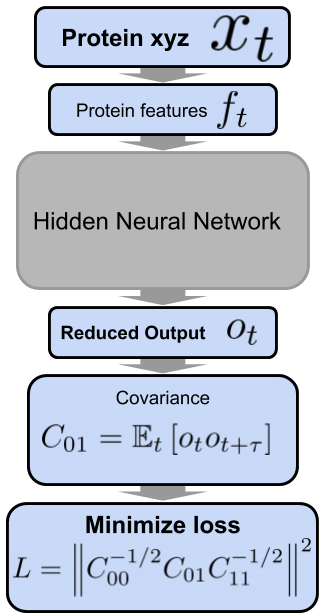
\includegraphics[width=0.4\linewidth]{figures3/NN.png}
  \caption{Schematics of the state-free reversible VAMPnets (SRV).}
  \label{fig:NN}
\end{figure}


crossvalidation  - lorenzo fig5 6.1


\section{MSM}

The first two variations (named $1/C_{M,1}^C$ and $1/C_{M,2}^C$) make use of the count
matrix $C_{ij}$ to directly estimate the on-the-fly MSM transition matrix. The count matrix
$C_{ij}$ contains the number of transitions that have been recorded in previous
iterations from state $i$ to state $j$. Every time a state is visited, the corresponding value
in the count matrix is incremented by one. This count matrix is normalized such
that each row sums to one and then used to estimate the on-the-fly MSM for the
adaptive sampling strategies.


check  lorenzo chapter 2
mfpt
eigenvectors

markovian property

implied timescales equation 3.12


The dimension reduced trajectories are then clustered with k-means into approximately 200 microstates,
the detailed values for each protein are provided in the Supplementary Information. 
A  maximum-likelihood estimation with a detailed balance
constraint \cite{prinz2011markov} allows obtaining an MSM transition matrix 
between every pair of microstates. All the analysis was
performed using the PyEMMA Python package \cite{scherer2015pyemma}, which
allows fast adjustments in the analysis step. The exact parameters for the MSM
construction for each protein are listed in the
Supplementary Information.


The analysis is summarized by a transition matrix,
$T_{ij}$, that indicates the probability that the system transitions from state
$i$ to state $j$ within a chosen lag time $\tau$. The discretization of the
original conformational space into states (also called microstates) is usually
performed by clustering the conformations sampled by MD trajectories using
a distance metric that can separate slowly mixing conformations from rapidly
interconverting ones \cite{noe2016commute, Noe2015}.


\section{energy landscape }
energy landscape 
folding funnel \cite{bryngelson1995p}
focker planck equation

Boltzmann distribution - lornezo
lronzeo fig 7.6

state space

state space $\varOmega\in\mathbb{R^{6n}}$, positions and momenta of the n atoms of the system)
[12]